%!TEX root = ../main.tex
\part{�tude 4 : Tensorpac, logiciel Python de calcul de Phase-Amplitude Coupling}
\label{Etude4_tensorpac}
\pagestyle{headings}


\chapter*{Introduction}
Le \pacFR (PAC) est un marqueur qui mesure le degr�s de couplage entre la phase d'ondes lentes et l'amplitude d'ondes rapides. L'�valuation d'un couplage se fait de mani�re suivante :
\begin{itemize}    
    \item Extraction de la phase et de l'amplitude en utilisant soit des outils de filtrage suivi de la transform�e d'Hilbert, soit une transformation continue en ondelettes.
    \item Calcul du couplage entre ces deux signaux en utilisant une des m�thodologies existantes \citep{tort_measuring_2010,ozkurt_statistically_2012,canolty_high_2006}...
    \item Le PAC �tant une mesure sensible aux bruits, on construit une distribution de mesure de PAC pouvant arriver par chance.
    \item La v�ritable mesure de PAC est ensuite normalis�e par cette distribution de chance afin de minimiser le bruit.
\end{itemize}
Un nombre cons�quent de m�thodes ont �t� propos�es pour chacune de ces �tapes ce qui complique la comparaison et la reproductibilit�. De plus, toutes les publications introduisant de nouvelles m�thodes les pr�sentent en utilisant des vecteurs et ne fournissent pas l'adaptation matricielle ce qui ne prend pas en compte le format des donn�es (nombre de sujets, d'�lectrodes, d'essais...) et donc n'est pas du tout optimal d'un point de vue temps de calcul.\\
Dans ce contexte, nous avons mis en place une toolbox Python, \textit{Tensorpac}, d�di�e exclusivement au calcul du \pacFR. Dans cette toolbox les m�thodes sont impl�ment�es de fa�on modulaire ce qui signifie que l'utilisateur peut combiner les m�thodes existantes pour chacune des �tapes du calcul du PAC. D'autre part, \textit{Tensorpac} utilise des tenseurs permettant de g�n�raliser le calcul � partir de s�ries temporelles vers des donn�es multi-dimensionnelles. Cette impl�mentation en tenseurs est combin�e � du calcul en parall�le ce qui diminue encore le temps d'ex�cution et facilite l'envoie sur des serveurs de calcul. Ce paquet inclue �galement le calcul de comodulograme (soit en cherchant les couples (phase, amplitude) soit en fixant l'un des deux et en faisant varier la largeur de bande de l'autre), statistiques et la visualisation. Pour finir, \textit{Tensorpac} est distribu� sous une licence BSD et peut �tre t�l�charger sur Github \footnotemark[1] et nous fournissons �galement une documentation d�taill�e \footnotemark[2].

\footnotetext[1]{\url{https://github.com/EtienneCmb/tensorpac}}
\footnotetext[2]{\url{https://etiennecmb.github.io/tensorpac/}}


%%% --------------------------
%%% Article
%%% --------------------------
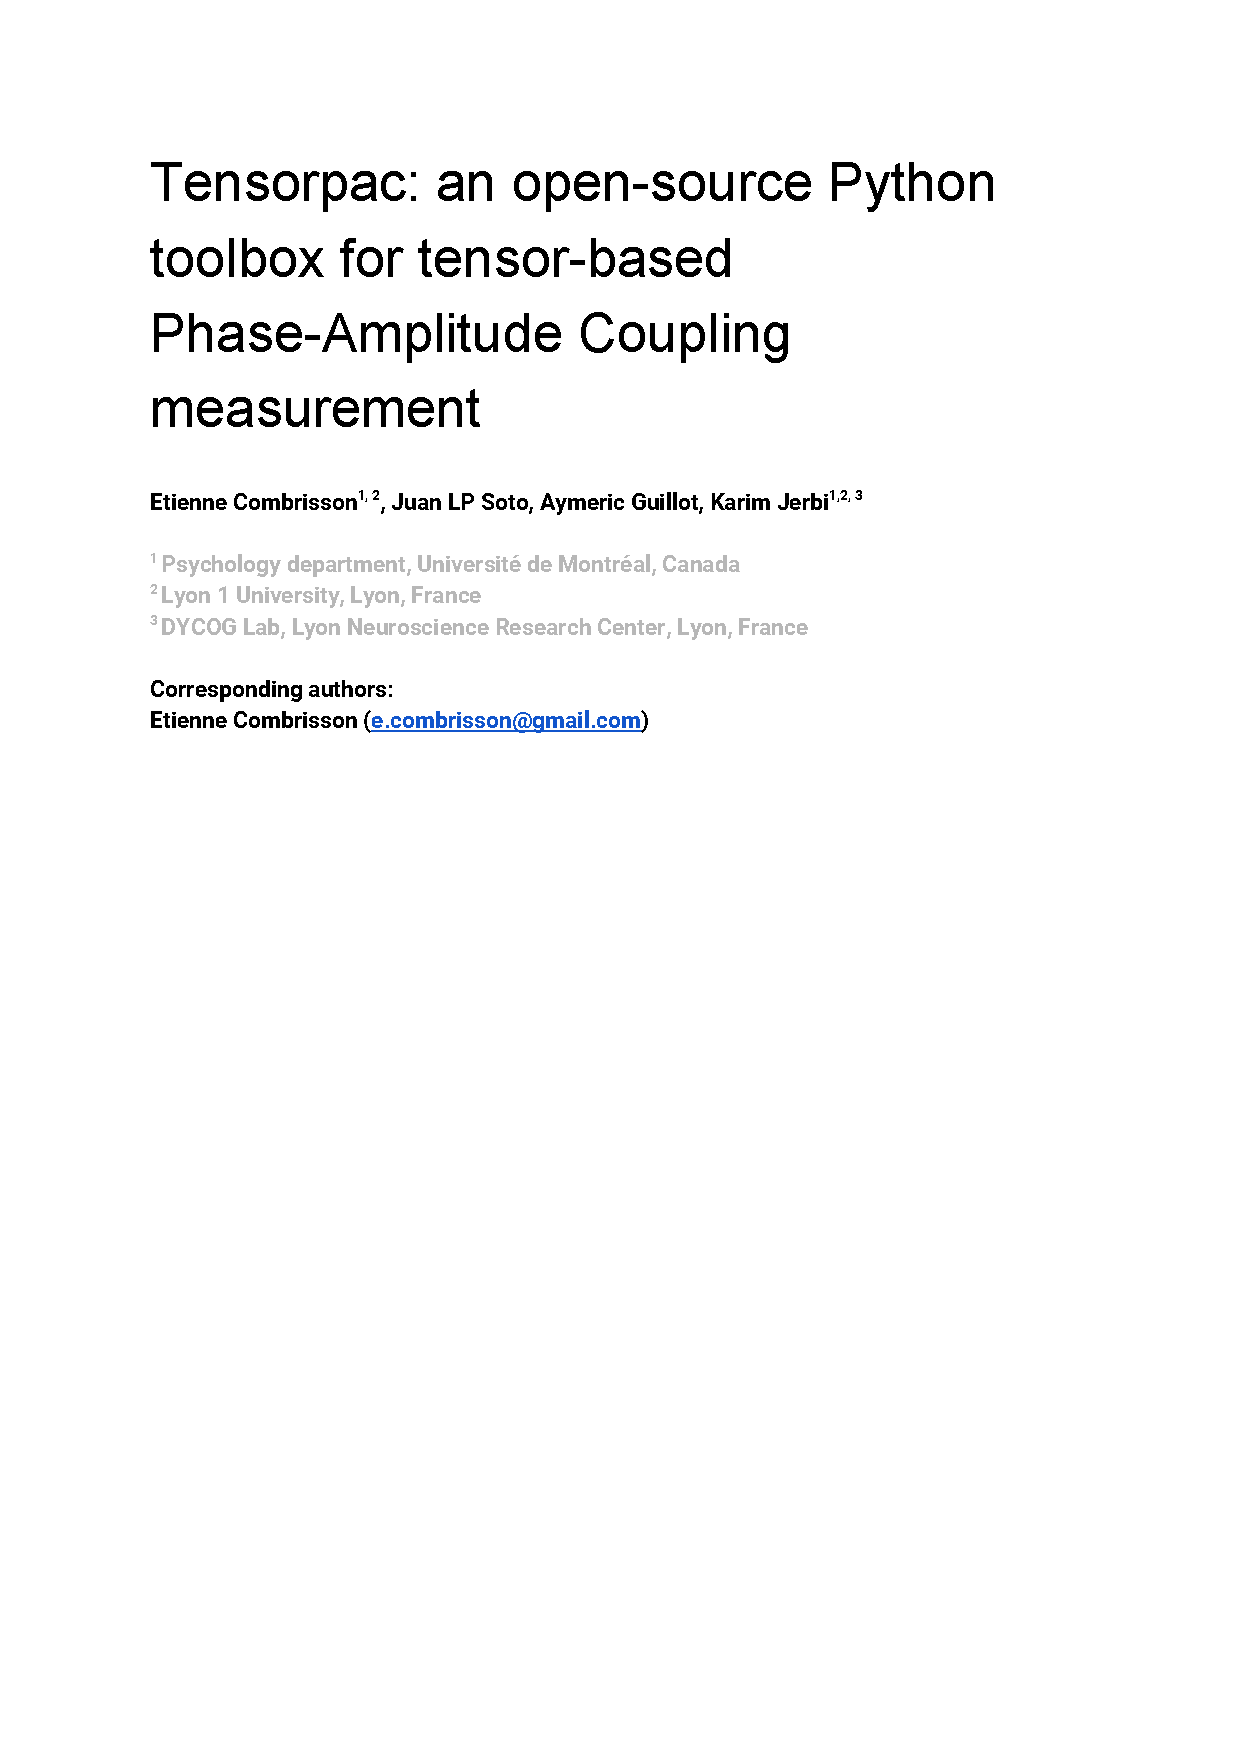
\includepdf[pages={1-18}]{Chap4/combrisson_2017_tensorpac.pdf}